\documentclass[11pt,aspectratio=169]{beamer}

\usepackage[utf8]{inputenc}
\usepackage[T1]{fontenc}
\usepackage[english]{babel}
\usepackage{amsmath, amssymb, amsfonts}
\usepackage{tikz}
\usetikzlibrary{positioning, shapes, arrows.meta}

% Theme
\usetheme{Madrid}
\usecolortheme{whale}
\setbeamertemplate{navigation symbols}{}
\setbeamertemplate{caption}[numbered]
\setbeamertemplate{footline}[frame number]

% Custom blocks
\setbeamercolor{block title}{bg=blue!70!black,fg=white}
\setbeamercolor{block body}{bg=blue!5,fg=black}
\setbeamercolor{block title alerted}{bg=red!70!black,fg=white}
\setbeamercolor{block body alerted}{bg=red!5,fg=black}
\setbeamercolor{block title example}{bg=green!50!black,fg=white}
\setbeamercolor{block body example}{bg=green!5,fg=black}

\title[Fundamentals of NLP]{Fundamentals of Natural Language Processing}
\subtitle{Part 1: NLP Landscape and Text Representation}
\author{Aymen Ben Brik}
\institute{M1 GAMMA \& L2 LMAD --- Data Science}
\date{\today}

\begin{document}

% =============================================================
% TITLE
% =============================================================
\begin{frame}
\titlepage
\end{frame}

% =============================================================
% OUTLINE
% =============================================================
\begin{frame}{Course outline}
\begin{columns}[T]
\begin{column}{0.5\textwidth}
\textbf{Chapter 1 --- NLP Landscape}
\begin{enumerate}
    \item What is NLP? Core challenges
    \item Major NLP tasks and applications
    \item NLP within the AI ecosystem
    \item Discriminative vs.\ generative models
    \item Historical evolution
\end{enumerate}
\end{column}
\begin{column}{0.5\textwidth}
\textbf{Chapter 2 --- Text Representation \& Evaluation}
\begin{enumerate}
    \setcounter{enumi}{5}
    \item Tokenization fundamentals
    \item Sparse representations: BoW, TF--IDF
    \item Dense representations: Word2Vec, GloVe, FastText
    \item Semantic similarity
    \item Evaluation metrics
\end{enumerate}
\end{column}
\end{columns}
\end{frame}

\begin{frame}{Learning objectives}
By the end of this course, you will be able to:
\begin{enumerate}
    \item \textbf{Define} NLP and identify its core challenges.
    \item \textbf{Recognize} the major NLP tasks and their applications.
    \item \textbf{Situate} NLP within the broader AI landscape.
    \item \textbf{Distinguish} discriminative from generative modelling.
    \item \textbf{Trace} the evolution from rules to LLMs.
    \item \textbf{Apply} tokenization and vector-space representations.
    \item \textbf{Compute} evaluation metrics adapted to each task.
\end{enumerate}
\end{frame}

% =============================================================
% CHAPTER 1
% =============================================================
\section{Chapter 1 --- NLP Landscape}

\begin{frame}
\centering
\Large \textbf{Chapter 1}\\[1em]
\large NLP Landscape\\[1em]
\normalsize Definition, tasks, paradigms and historical evolution
\end{frame}

\subsection{What is NLP?}

\begin{frame}{What is Natural Language Processing?}
\begin{block}{Definition}
NLP is the subfield of AI that builds systems able to \textbf{process}, \textbf{understand} and \textbf{generate} human language. It sits at the intersection of \emph{linguistics}, \emph{computer science} and \emph{machine learning}.
\end{block}
\vfill
\textbf{Three axes:}
\begin{itemize}
    \item \textbf{NLU} --- understanding: extract meaning, entities, sentiment.
    \item \textbf{NLG} --- generation: produce fluent, coherent text.
    \item \textbf{Interaction} --- dialogue and conversational agents.
\end{itemize}
\end{frame}

\begin{frame}{Why is natural language hard?}
\begin{columns}[T]
\begin{column}{0.5\textwidth}
\begin{alertblock}{Ambiguity}
\begin{itemize}
    \item \textbf{Lexical}: ``\emph{bank}'' (money / river)
    \item \textbf{Syntactic}: ``\emph{I saw the man with the telescope.}''
    \item \textbf{Semantic}: ``\emph{The chicken is ready to eat.}''
    \item \textbf{Pragmatic}: ``\emph{Can you pass the salt?}''
\end{itemize}
\end{alertblock}
\end{column}
\begin{column}{0.5\textwidth}
\begin{alertblock}{Context dependence}
\begin{itemize}
    \item Same word, different referents (\emph{Apple})
    \item Pronoun resolution
    \item Sarcasm, irony
\end{itemize}
\end{alertblock}
\begin{alertblock}{Variability}
\begin{itemize}
    \item Synonymy, paraphrasing
    \item Spelling variation, slang
    \item Code-switching, dialects
\end{itemize}
\end{alertblock}
\end{column}
\end{columns}
\end{frame}

\begin{frame}{The headline that everyone misreads}
\textbf{Real headline:}
\begin{quote}
``\emph{Stolen painting found by tree.}''
\end{quote}
\vfill
\textbf{Two grammatical readings:}
\begin{enumerate}
    \item \emph{found by [tree]} --- a tree found the painting (absurd).
    \item \emph{found [by tree]} --- the painting was found beside a tree (likely).
\end{enumerate}
\vfill
\begin{exampleblock}{Lesson}
World knowledge (trees are inanimate) lets us discard reading 1. A computer without such knowledge cannot disambiguate without an explicit mechanism. This is the central challenge NLP must solve.
\end{exampleblock}
\end{frame}

\subsection{Major NLP tasks}

\begin{frame}{A taxonomy by input--output structure}
\begin{center}
\begin{tabular}{|l|l|l|}
\hline
\textbf{Category} & \textbf{Input} & \textbf{Output} \\
\hline
Text classification & text & discrete label(s) \\
Sequence labelling & text & one label per token \\
Sequence-to-sequence & text & a different text \\
Question answering & question + context & answer (span / text) \\
Open-ended generation & prompt & arbitrary text \\
\hline
\end{tabular}
\end{center}
\vfill
\textbf{Spectrum of output complexity:} from one integer (classification) to free-form sequences (generation). Each level adds expressiveness and evaluation difficulty.
\end{frame}

\begin{frame}{Classification \& sequence labelling}
\begin{columns}[T]
\begin{column}{0.5\textwidth}
\begin{block}{Text classification}
\textbf{One label per document.}
\begin{itemize}
    \item Sentiment analysis
    \item Spam detection
    \item Topic categorization
    \item Intent detection (chatbot)
    \item Toxicity / hate speech
\end{itemize}
\end{block}
\end{column}
\begin{column}{0.5\textwidth}
\begin{block}{Sequence labelling}
\textbf{One label per token.}
\begin{itemize}
    \item POS tagging
    \item Named Entity Recognition (NER)
    \item Slot filling
\end{itemize}
\textbf{B-I-O scheme:}\\
\emph{Apple/B-ORG was/O founded/O by/O Steve/B-PER Jobs/I-PER}
\end{block}
\end{column}
\end{columns}
\end{frame}

\begin{frame}{Generation tasks}
\begin{columns}[T]
\begin{column}{0.5\textwidth}
\begin{block}{Sequence-to-sequence}
\begin{itemize}
    \item Machine translation
    \item Abstractive summarization
    \item Paraphrasing
    \item Grammar correction
\end{itemize}
\end{block}
\end{column}
\begin{column}{0.5\textwidth}
\begin{block}{Question answering}
\begin{itemize}
    \item \textbf{Extractive}: span in context
    \item \textbf{Closed-book}: no context
    \item \textbf{Open-domain}: retrieve + read (RAG)
    \item \textbf{Generative}
\end{itemize}
\end{block}
\end{column}
\end{columns}
\vfill
\begin{exampleblock}{Open-ended generation}
The regime of large language models (LLMs): given a prompt, produce a fluent continuation. Evaluation is intrinsically harder because many outputs are acceptable.
\end{exampleblock}
\end{frame}

\subsection{NLP in the AI ecosystem}

\begin{frame}{The AI / ML / DL hierarchy}
\begin{center}
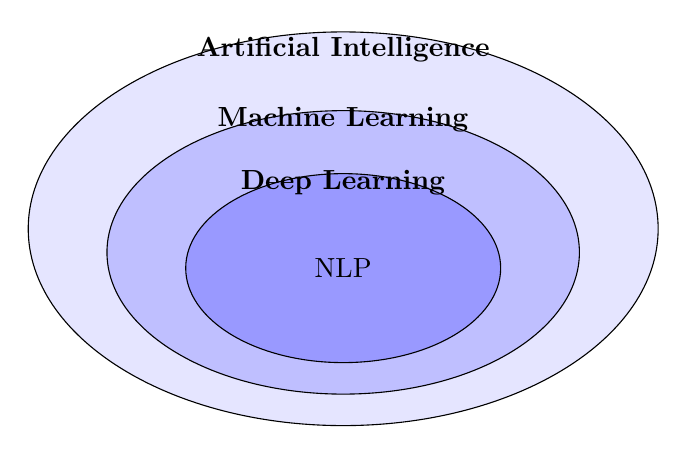
\begin{tikzpicture}
\draw[fill=blue!10] (0,0) ellipse (4 and 2.5) node[above=2.0cm] {\textbf{Artificial Intelligence}};
\draw[fill=blue!25] (0,-0.3) ellipse (3 and 1.8) node[above=1.4cm] {\textbf{Machine Learning}};
\draw[fill=blue!40] (0,-0.5) ellipse (2 and 1.2) node[above=0.8cm] {\textbf{Deep Learning}};
\node at (0,-0.5) {NLP};
\end{tikzpicture}
\end{center}
\vfill
\textbf{Strict inclusion:} $\mathrm{DL} \subset \mathrm{ML} \subset \mathrm{AI}$. NLP is a domain that draws on all three across its history.
\end{frame}

\begin{frame}{The four ingredients of any learned system}
\begin{block}{Learning quadruple $(D, \mathcal{F}, \mathcal{L}, \mathcal{O})$}
\begin{itemize}
    \item \textbf{Data} $D = \{(x_i, y_i)\}_{i=1}^N$ --- training examples.
    \item \textbf{Model} $\mathcal{F} = \{f_\theta : \theta \in \Theta\}$ --- parameterised functions.
    \item \textbf{Loss} $\mathcal{L}(\hat{y}, y)$ --- penalty for bad predictions.
    \item \textbf{Optimizer} $\mathcal{O}$ --- updates $\theta$ to reduce average loss.
\end{itemize}
\end{block}
\vfill
\textbf{Empirical Risk Minimization:}
\[ \theta^* \in \arg\min_{\theta} \frac{1}{N} \sum_{i=1}^{N} \mathcal{L}\big(f_\theta(x_i), y_i\big). \]
\end{frame}

\begin{frame}{Three learning paradigms}
\begin{center}
\begin{tabular}{|l|l|l|l|}
\hline
\textbf{Paradigm} & \textbf{Labels?} & \textbf{Goal} & \textbf{NLP example} \\
\hline
Supervised & Provided & Predict $y \mid x$ & Spam detection \\
Unsupervised & None & Find structure & Topic clustering \\
Self-supervised & Manufactured & Learn representations & Next-token prediction \\
\hline
\end{tabular}
\end{center}
\vfill
\begin{block}{Why self-supervision dominates modern NLP}
Self-supervised pretraining converts \emph{any} large unlabelled text into a training signal. The model learns general linguistic competence and transfers to downstream tasks via fine-tuning or prompting.
\end{block}
\end{frame}

\subsection{Discriminative vs.\ generative}

\begin{frame}{Discriminative vs.\ generative}
\begin{columns}[T]
\begin{column}{0.5\textwidth}
\begin{block}{Discriminative}
Models $P(y \mid x)$.
\begin{itemize}
    \item Decision boundary
    \item LR, SVM, BERT, CRF
    \item Predicts labels directly
    \item Cannot generate text
\end{itemize}
\end{block}
\end{column}
\begin{column}{0.5\textwidth}
\begin{block}{Generative}
Models $P(x)$ or $P(x, y)$.
\begin{itemize}
    \item Distribution over inputs
    \item N-grams, GPT, T5, VAEs
    \item Can generate samples
    \item Can score likelihoods
\end{itemize}
\end{block}
\end{column}
\end{columns}
\vfill
\begin{exampleblock}{Bayes bridge (one-way)}
Generative $\Rightarrow$ Discriminative via $P(y \mid x) = \frac{P(x \mid y) P(y)}{\sum_{y'} P(x \mid y') P(y')}$.
The reverse direction is impossible.
\end{exampleblock}
\end{frame}

\begin{frame}{The modern blur}
\begin{alertblock}{LLMs are generative models doing discriminative tasks}
A decoder-only Transformer (GPT-4, Claude, LLaMA) is trained generatively (next-token prediction) but can be \emph{prompted} to solve any classification task:
\begin{quote}
``\emph{Classify the following review as positive or negative: \dots}''
\end{quote}
The model produces the answer as a continuation, exploiting its general linguistic competence.
\end{alertblock}
\vfill
$\Rightarrow$ A single generative model handles the full task taxonomy.
\end{frame}

\subsection{Historical evolution}

\begin{frame}{Four eras of NLP}
\begin{center}
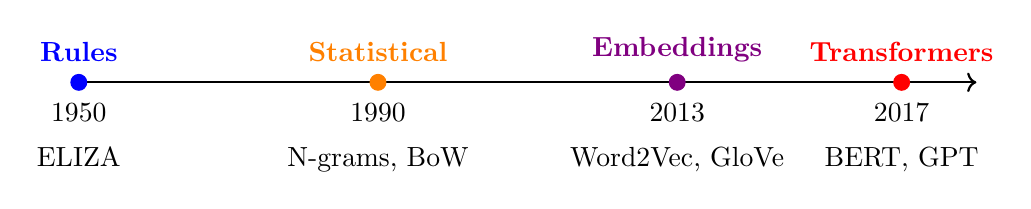
\begin{tikzpicture}[scale=0.95]
\draw[->, thick] (0,0) -- (12,0);
\foreach \x/\year/\era/\col in {0/1950/Rules/blue, 4/1990/Statistical/orange, 8/2013/Embeddings/violet, 11/2017/Transformers/red}{
    \filldraw[\col] (\x,0) circle (3pt);
    \node[above=4pt, \col] at (\x,0) {\textbf{\era}};
    \node[below=4pt] at (\x,0) {\year};
}
\node[below=20pt] at (0,0) {ELIZA};
\node[below=20pt] at (4,0) {N-grams, BoW};
\node[below=20pt] at (8,0) {Word2Vec, GloVe};
\node[below=20pt] at (11,0) {BERT, GPT};
\end{tikzpicture}
\end{center}
\vfill
\begin{block}{Recurring pattern}
Each era \textbf{addresses the previous one's failure mode}: rules don't scale $\to$ statistics; counts lack semantics $\to$ embeddings; embeddings are static $\to$ contextualisation.
\end{block}
\end{frame}

\begin{frame}{Era 1 --- Rule-based (1950--1980)}
\begin{itemize}
    \item Linguists hand-write rules; expert systems encode facts.
    \item Formal grammars, regex, dictionary-based morphological analysers.
    \item Examples: ELIZA (1966), SHRDLU (1972), Georgetown--IBM MT (1954).
\end{itemize}
\vfill
\begin{alertblock}{Limitations}
Brittle, language-specific, expensive maintenance, cannot handle ambiguity probabilistically.
\end{alertblock}
\end{frame}

\begin{frame}{Era 2 --- Statistical (1990--2010)}
\begin{block}{N-gram language model}
\[ P(w_1, \dots, w_T) \approx \prod_{t=1}^{T} P(w_t \mid w_{t-n+1}, \dots, w_{t-1}). \]
Probabilities estimated by counting in a corpus.
\end{block}
\begin{itemize}
    \item Hidden Markov Models for POS tagging.
    \item Bag-of-Words, TF--IDF for retrieval.
    \item Maximum-entropy and log-linear classifiers.
\end{itemize}
\begin{alertblock}{Limitations}
Sparse data, fixed context window, no semantic similarity.
\end{alertblock}
\end{frame}

\begin{frame}{Era 3 --- Word embeddings (2013--2017)}
\begin{block}{Idea}
Each word $\to$ a dense vector in $\mathbb{R}^d$ (typically $d = 50$--$300$). Words with similar contexts get similar vectors.
\end{block}
\begin{itemize}
    \item \textbf{Word2Vec} (Mikolov 2013): skip-gram, CBOW.
    \item \textbf{GloVe} (Pennington 2014): co-occurrence matrix factorization.
    \item \textbf{FastText} (Bojanowski 2017): sub-word $n$-grams, no OOV.
\end{itemize}
\begin{exampleblock}{Vector arithmetic}
$\overrightarrow{\text{king}} - \overrightarrow{\text{man}} + \overrightarrow{\text{woman}} \approx \overrightarrow{\text{queen}}$
\end{exampleblock}
\begin{alertblock}{Limitations}
Static (one vector per word, regardless of context).
\end{alertblock}
\end{frame}

\begin{frame}{Era 4 --- Transformers \& LLMs (2017--)}
\begin{itemize}
    \item Vaswani et al.\ (2017): \emph{``Attention Is All You Need''}.
    \item BERT (2018): masked LM, encoder-only, fine-tuned downstream.
    \item GPT-1, 2, 3, 4: causal LM, decoder-only, scaled to billions of parameters.
\end{itemize}
\vfill
\begin{block}{Hallmarks}
\textbf{Contextual} embeddings $\bullet$ \textbf{self-supervised} pretraining at Web scale $\bullet$ \textbf{foundation} models adapted to many tasks $\bullet$ \textbf{scaling laws} $\bullet$ chain-of-thought reasoning $\bullet$ RLHF alignment.
\end{block}
\end{frame}

% =============================================================
% CHAPTER 2
% =============================================================
\section{Chapter 2 --- Text Representation \& Evaluation}

\begin{frame}
\centering
\Large \textbf{Chapter 2}\\[1em]
\large Text Representation and Evaluation\\[1em]
\normalsize From raw text to vectors and metrics
\end{frame}

\subsection{Tokenization}

\begin{frame}{Tokenization: the first critical step}
\begin{block}{Why tokenize?}
Models cannot process raw text directly. Tokenization converts text into \textbf{discrete units} that can be represented numerically.
\end{block}
\vfill
\begin{center}
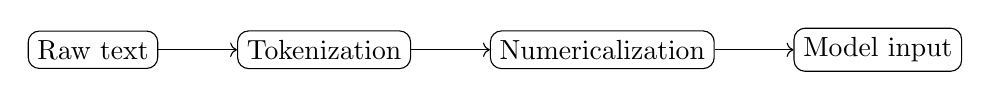
\begin{tikzpicture}[node distance=1cm]
\node[draw, rounded corners] (a) {Raw text};
\node[draw, rounded corners, right=of a] (b) {Tokenization};
\node[draw, rounded corners, right=of b] (c) {Numericalization};
\node[draw, rounded corners, right=of c] (d) {Model input};
\draw[->] (a) -- (b);
\draw[->] (b) -- (c);
\draw[->] (c) -- (d);
\end{tikzpicture}
\end{center}
\vfill
\textbf{``I love NLP''} $\to$ \texttt{[I, love, NLP]} $\to$ \texttt{[42, 318, 7953]}
\end{frame}

\begin{frame}{Three granularities}
\begin{center}
\begin{tabular}{|l|l|l|l|}
\hline
\textbf{Level} & \textbf{Vocab size} & \textbf{Sequence length} & \textbf{OOV} \\
\hline
Word & Very large ($10^5$--$10^6$) & Short & \texttt{[UNK]} \\
Character & Tiny ($\sim 100$) & Very long & None \\
Sub-word (BPE) & Moderate ($10^4$--$10^5$) & Moderate & Robust \\
\hline
\end{tabular}
\end{center}
\vfill
\begin{block}{Modern LLMs}
GPT, BERT, LLaMA --- all use \textbf{sub-word} tokenization (BPE, WordPiece, SentencePiece). Best trade-off between vocabulary size and sequence length.
\end{block}
\end{frame}

\begin{frame}{Byte-Pair Encoding (BPE)}
\textbf{Algorithm:}
\begin{enumerate}
    \item Start with character-level vocabulary.
    \item Count adjacent symbol pairs in the corpus.
    \item Merge the most frequent pair into a new symbol.
    \item Repeat until vocabulary reaches target size.
\end{enumerate}
\vfill
\begin{exampleblock}{Example merge}
Corpus: \texttt{newest, newest, widest, lowest}\\
Most frequent pair: \texttt{e + s} $\to$ merge into \texttt{es}.\\
Then: \texttt{es + t} $\to$ \texttt{est}, etc.
\end{exampleblock}
\textbf{New word} \texttt{lowest} tokenizes as \texttt{low + est} (sub-words seen during training).
\end{frame}

\subsection{Sparse representations}

\begin{frame}{Bag-of-Words and TF--IDF}
\begin{columns}[T]
\begin{column}{0.5\textwidth}
\begin{block}{Bag-of-Words}
Document $\to$ vector of word \textbf{counts}.\\
\emph{``the cat sat''} $\to$ $[1, 1, 1, 0, \dots]$
\end{block}
\begin{block}{TF--IDF}
Down-weight common words, up-weight rare ones:
\[ \mathrm{tfidf}(w, d) = \mathrm{tf}(w, d) \times \log\frac{N}{\mathrm{df}(w)}. \]
\end{block}
\end{column}
\begin{column}{0.5\textwidth}
\begin{block}{Properties}
\begin{itemize}
    \item Simple, fast, interpretable
    \item Strong baseline for classification \& search
    \item Works well on small corpora
\end{itemize}
\end{block}
\begin{alertblock}{Limitations}
\begin{itemize}
    \item No word order
    \item No semantic similarity (\emph{cat $\bot$ kitten})
    \item Very high dimension
\end{itemize}
\end{alertblock}
\end{column}
\end{columns}
\end{frame}

\subsection{Dense representations}

\begin{frame}{Word2Vec --- distributional hypothesis}
\begin{block}{Distributional hypothesis (Firth, 1957)}
\emph{``You shall know a word by the company it keeps.''}\\
Words appearing in similar contexts have similar meanings.
\end{block}
\vfill
\begin{columns}[T]
\begin{column}{0.5\textwidth}
\textbf{Skip-gram}\\
Centre $\to$ predict context\\
\centering
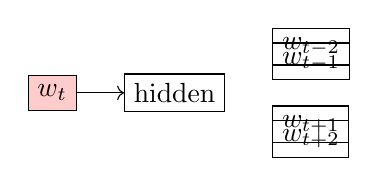
\begin{tikzpicture}[node distance=0.6cm]
\node[draw,fill=red!20] (c) {$w_t$};
\node[draw, right=of c] (h) {hidden};
\node[draw, above right=0.1cm and 0.6cm of h] {$w_{t-2}$};
\node[draw, right=of h, yshift=0.4cm] {$w_{t-1}$};
\node[draw, right=of h, yshift=-0.4cm] {$w_{t+1}$};
\node[draw, below right=0.1cm and 0.6cm of h] {$w_{t+2}$};
\draw[->] (c) -- (h);
\end{tikzpicture}
\end{column}
\begin{column}{0.5\textwidth}
\textbf{CBOW}\\
Context $\to$ predict centre\\
\centering
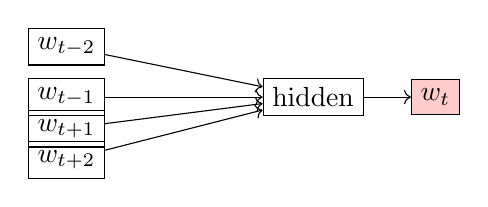
\begin{tikzpicture}[node distance=0.6cm]
\node[draw, above] (a) at (0,0.6) {$w_{t-2}$};
\node[draw] (b) at (0, 0.2) {$w_{t-1}$};
\node[draw] (c) at (0,-0.2) {$w_{t+1}$};
\node[draw] (d) at (0,-0.6) {$w_{t+2}$};
\node[draw, right=2cm of b] (h) {hidden};
\node[draw, fill=red!20, right=of h] (t) {$w_t$};
\draw[->] (a) -- (h);
\draw[->] (b) -- (h);
\draw[->] (c) -- (h);
\draw[->] (d) -- (h);
\draw[->] (h) -- (t);
\end{tikzpicture}
\end{column}
\end{columns}
\end{frame}

\begin{frame}{From rules to embeddings: a synthetic comparison}
\begin{center}
\small
\begin{tabular}{|l|l|l|l|l|}
\hline
\textbf{Approach} & \textbf{Representation} & \textbf{Semantics} & \textbf{Scalability} & \textbf{Era} \\
\hline
Rules & Symbolic & Manual & Low & 1950 \\
N-grams / BoW & Counts & No & Medium & 1990 \\
TF--IDF & Weighted counts & Partial & Medium & 1990 \\
Word2Vec & Dense vectors & Yes & High & 2013 \\
GloVe & Dense vectors & Yes & High & 2014 \\
FastText & Sub-word vectors & Yes & High & 2017 \\
Transformers & Contextual vectors & Yes & Very high & 2017+ \\
\hline
\end{tabular}
\end{center}
\vfill
\begin{block}{Next: contextual embeddings}
The static-vs-contextual distinction motivates the move to Transformers (Part 2 of this course).
\end{block}
\end{frame}

\subsection{Semantic similarity}

\begin{frame}{Measuring similarity}
\begin{columns}[T]
\begin{column}{0.5\textwidth}
\begin{block}{Cosine (most common)}
\[ \cos(\mathbf{a}, \mathbf{b}) = \frac{\mathbf{a}^\top \mathbf{b}}{\|\mathbf{a}\|\, \|\mathbf{b}\|} \in [-1, 1] \]
\textbf{Magnitude-invariant.} Preferred for text.
\end{block}
\begin{block}{Dot product}
\[ \mathbf{a}^\top \mathbf{b} \]
Fast; sensitive to magnitude.
\end{block}
\end{column}
\begin{column}{0.5\textwidth}
\begin{block}{Euclidean}
\[ d_2(\mathbf{a}, \mathbf{b}) = \|\mathbf{a} - \mathbf{b}\|_2 \]
Sensitive to magnitude AND direction.
\end{block}
\begin{exampleblock}{Rule of thumb}
Use cosine for text/TF--IDF/embeddings.\\
Use Euclidean for $k$-means after $\ell_2$-normalisation.\\
Use dot product for speed (after normalisation, equivalent to cosine).
\end{exampleblock}
\end{column}
\end{columns}
\end{frame}

\begin{frame}{The retrieval pattern}
\begin{center}
\large
\fbox{\parbox{0.8\textwidth}{\centering
$\text{query} \xrightarrow[\text{embed}]{} \mathbf{q} \xrightarrow[\text{nearest neighbours}]{} \text{top-}k \text{ docs}$}}
\end{center}
\vfill
\textbf{Applications:}
\begin{itemize}
    \item Semantic search engines
    \item Document deduplication
    \item Recommendation systems
    \item \textbf{Retrieval-augmented generation (RAG)} for LLMs
    \item Cross-lingual matching
\end{itemize}
\vfill
At scale: approximate nearest-neighbour libraries (FAISS, HNSW, ScaNN).
\end{frame}

\subsection{Evaluation metrics}

\begin{frame}{Why measure?}
\begin{quote}
\emph{``What is not measured cannot be improved.''}
\end{quote}
\vfill
\begin{columns}[T]
\begin{column}{0.5\textwidth}
\begin{block}{Classification (discriminative)}
\begin{itemize}
    \item Accuracy
    \item Precision, Recall
    \item F$_1$ score
\end{itemize}
\end{block}
\end{column}
\begin{column}{0.5\textwidth}
\begin{block}{Generation (generative)}
\begin{itemize}
    \item Perplexity (language modelling)
    \item BLEU (translation)
    \item ROUGE (summarisation)
\end{itemize}
\end{block}
\end{column}
\end{columns}
\vfill
\begin{alertblock}{Important}
No single metric tells the whole story. Always report several and consider the task context.
\end{alertblock}
\end{frame}

\begin{frame}{Classification metrics}
\begin{columns}[T]
\begin{column}{0.5\textwidth}
\begin{block}{Confusion matrix}
\begin{tabular}{|c|cc|}
\hline
& Pred + & Pred -- \\
\hline
True + & TP & FN \\
True -- & FP & TN \\
\hline
\end{tabular}
\end{block}
\begin{block}{Formulas}
\begin{align*}
\mathrm{Accuracy} &= \frac{\mathrm{TP} + \mathrm{TN}}{\mathrm{Total}} \\
\mathrm{Precision} &= \frac{\mathrm{TP}}{\mathrm{TP} + \mathrm{FP}} \\
\mathrm{Recall} &= \frac{\mathrm{TP}}{\mathrm{TP} + \mathrm{FN}}
\end{align*}
\end{block}
\end{column}
\begin{column}{0.5\textwidth}
\begin{block}{F$_1$ score}
Harmonic mean of P and R:
\[ F_1 = 2 \cdot \frac{P \cdot R}{P + R} \]
High only when \textbf{both} are high.
\end{block}
\begin{alertblock}{Class imbalance!}
With 95\% negative examples, ``always predict negative'' achieves 95\% accuracy --- but is useless.\\
$\Rightarrow$ Always inspect P, R, F$_1$.
\end{alertblock}
\end{column}
\end{columns}
\end{frame}

\begin{frame}{Precision vs Recall: which to optimize?}
\begin{block}{Library analogy}
\textbf{Precision}: of the books I brought home, how many are about ML?\\
\textbf{Recall}: of all ML books in the library, how many did I bring home?
\end{block}
\vfill
\begin{columns}[T]
\begin{column}{0.33\textwidth}
\begin{block}{High Precision}
Spam detection\\
Legal search
\end{block}
\end{column}
\begin{column}{0.33\textwidth}
\begin{block}{High Recall}
Medical screening\\
Fraud detection
\end{block}
\end{column}
\begin{column}{0.33\textwidth}
\begin{block}{Balanced (F$_1$)}
NER\\
Sentiment\\
Most NLP tasks
\end{block}
\end{column}
\end{columns}
\end{frame}

\begin{frame}{Perplexity --- evaluating language models}
\begin{block}{Definition}
\[ \mathrm{PPL} = \exp\!\left( - \frac{1}{N} \sum_{i=1}^{N} \log P(w_i \mid w_1, \dots, w_{i-1}) \right). \]
\end{block}
\vfill
\textbf{Intuition:} If $\mathrm{PPL} = k$, the model is on average ``hesitating between $k$ equally likely words'' at each position.
\vfill
\textbf{Lower is better.} $\mathrm{PPL} = 1$ means perfect prediction.
\vfill
\begin{alertblock}{Caveat}
Low perplexity does \textbf{not} guarantee high-quality generation. A model can be confident yet repetitive.
\end{alertblock}
\end{frame}

\begin{frame}{BLEU --- evaluating translation}
\textbf{B}ilingual \textbf{E}valuation \textbf{U}nderstudy (Papineni et al., 2002).
\begin{block}{Formula}
\[ \mathrm{BLEU} = \mathrm{BP} \cdot \exp\!\left( \frac{1}{N} \sum_{n=1}^{N} \log p_n \right), \]
\end{block}
where:
\begin{itemize}
    \item $p_n$ = modified $n$-gram precision (capped by reference counts).
    \item $\mathrm{BP}$ = brevity penalty (penalises too-short outputs).
\end{itemize}
\vfill
\begin{exampleblock}{Quick example}
Reference: \emph{The cat sat on the mat.}\\
Candidate: \emph{The cat sat on the mat.} $\to$ BLEU = 1.0\\
Candidate: \emph{The cat on the mat.} $\to$ BLEU drops (missing word).
\end{exampleblock}
\end{frame}

\begin{frame}{ROUGE --- evaluating summarisation}
\textbf{R}ecall-\textbf{O}riented \textbf{U}nderstudy for \textbf{G}isting \textbf{E}valuation (Lin, 2004).
\begin{columns}[T]
\begin{column}{0.5\textwidth}
\begin{block}{ROUGE-N}
\[ \frac{|\,n\text{-grams}_c \cap n\text{-grams}_r\,|}{|\,n\text{-grams}_r\,|} \]
\begin{itemize}
    \item ROUGE-1: unigrams
    \item ROUGE-2: bigrams
\end{itemize}
\end{block}
\end{column}
\begin{column}{0.5\textwidth}
\begin{block}{ROUGE-L}
Based on the longest common subsequence (LCS).\\[0.3em]
Captures sentence-level structure without requiring contiguous matches.
\end{block}
\end{column}
\end{columns}
\vfill
\begin{exampleblock}{BLEU vs ROUGE}
\textbf{BLEU} = precision-oriented (translation).\\
\textbf{ROUGE} = recall-oriented (summarisation, where missing content is the failure mode).
\end{exampleblock}
\end{frame}

\begin{frame}{Metrics summary}
\begin{center}
\small
\begin{tabular}{|l|l|l|l|}
\hline
\textbf{Metric} & \textbf{Task} & \textbf{Measures} & \textbf{Range} \\
\hline
Accuracy & Classification & Overall correctness & $[0, 1]$ \\
Precision & Classification & Prediction quality & $[0, 1]$ \\
Recall & Classification & Coverage & $[0, 1]$ \\
F$_1$ & Classification & Harmonic mean P/R & $[0, 1]$ \\
Perplexity & Language modelling & Predictive quality & $[1, \infty)$ \\
BLEU & Translation & $n$-gram precision & $[0, 1]$ \\
ROUGE-N & Summarisation & $n$-gram recall & $[0, 1]$ \\
ROUGE-L & Summarisation & LCS recall & $[0, 1]$ \\
\hline
\end{tabular}
\end{center}
\vfill
\begin{block}{Modern complementary metrics}
\textbf{BERTScore} (semantic), \textbf{LLM-as-a-judge}, \textbf{RAGAS} (RAG eval), \textbf{MT-Bench} (instructions).
\end{block}
\end{frame}

% =============================================================
% CONCLUSION
% =============================================================
\section*{Conclusion}

\begin{frame}{Take-aways}
\begin{enumerate}
    \item NLP is hard because of \textbf{ambiguity}, \textbf{context}, and \textbf{variability}.
    \item Tasks span \textbf{classification, sequence labelling, seq-to-seq, QA, generation}.
    \item NLP draws on \textbf{ML and DL}; modern systems are \textbf{self-supervised} and generative.
    \item Each historical era \textbf{addressed the previous one's failure mode}.
    \item Tokenization, vector representations and metrics are the \textbf{core toolkit} every practitioner must master.
\end{enumerate}
\end{frame}

\begin{frame}{What's next?}
\begin{block}{Lab notebooks (4 sessions)}
\begin{itemize}
    \item \texttt{lab01-tokenization.ipynb}
    \item \texttt{lab02-bow-tfidf-classifier.ipynb}
    \item \texttt{lab03-word2vec-embeddings.ipynb}
    \item \texttt{lab04-evaluation-metrics.ipynb}
\end{itemize}
\end{block}
\vfill
\begin{block}{Future parts}
\textbf{Part 2:} From RNNs to Transformers (sequence models, attention, BERT, GPT)\\
\textbf{Part 3:} Pretraining and fine-tuning (transfer learning, instruction tuning, RLHF)\\
\textbf{Part 4:} Retrieval-Augmented Generation (RAG) and AI agents
\end{block}
\end{frame}

\begin{frame}
\centering
\Huge \textbf{Thank you!}\\[1em]
\large Questions?\\[1em]
\normalsize \texttt{https://github.com/Aymenbenbrik/FundamentalsNLP}
\end{frame}

\end{document}
